\documentclass[a4paper,12pt]{article} %размер бумаги устанавливаем А4, шрифт 12пунктов
\usepackage[T2A]{fontenc}
\usepackage[english, french, russian]{babel}
\usepackage[utf8]{inputenc}


\usepackage{amsmath}
\usepackage{amsthm}
\usepackage{amssymb}
\usepackage{fancyhdr}
\usepackage{graphicx}
\usepackage{colortbl}
\usepackage{tikz}
\usepackage{pgf}
\usepackage{subcaption}
\usepackage{listings}
\usepackage[colorlinks,urlcolor=blue]{hyperref}

\parindent=1cm
\usepackage{indentfirst}

% \renewcommand{\rmdefault}{ftm} % Times New Roman
\graphicspath{{images/}} %путь к рисункам

\makeatletter
\renewcommand{\@biblabel}[1]{#1.} % Заменяем библиографию с квадратных скобок на точку:
\makeatother

\usepackage{geometry} % Меняем поля страницы
\geometry{left=2.5cm}% левое поле
\geometry{right=1.5cm}% правое поле
\geometry{top=1.5cm}% верхнее поле
\geometry{bottom=1.5cm}% нижнее поле
\renewcommand{\baselinestretch}{1.5} % междустрочный интервал


\newcommand{\bibref}[3]{\hyperlink{#1}{#2 (#3)}} % biblabel, authors, year

\renewcommand{\theenumi}{\arabic{enumi}}% Меняем везде перечисления на цифра.цифра
\renewcommand{\labelenumi}{\arabic{enumi}}% Меняем везде перечисления на цифра.цифра
\renewcommand{\theenumii}{.\arabic{enumii}}% Меняем везде перечисления на цифра.цифра
\renewcommand{\labelenumii}{\arabic{enumi}.\arabic{enumii}.}% Меняем везде перечисления на цифра.цифра
\renewcommand{\theenumiii}{.\arabic{enumiii}}% Меняем везде перечисления на цифра.цифра
\renewcommand{\labelenumiii}{\arabic{enumi}.\arabic{enumii}.\arabic{enumiii}.}% Меняем везде перечисления на цифра.цифра

\newcommand{\imgh}[3]{\begin{figure}[h]\center{\includegraphics[width=#1]{#2}}\caption{#3}\label{ris:#2}\end{figure}}

\begin{document}
	% Титульный лист -----------------------------
	\begin{titlepage}
\newpage

\begin{center}
Федеральное государственное автономное образовательное учреждение высшего образования "Национальный исследовательский университет "Высшая школа экономики"
\\
\medskip
Факультет компьютерных наук \\
Основная образовательная программа \\
Прикладная математика и информатика \\
\end{center}

\vspace{8em}

\begin{center}
\Large КУРСОВАЯ РАБОТА \\
\end{center}

\vspace{2em}

\begin{center}
\textsc{\textbf{
Исследовательский проект на тему
\linebreak
"Оценка неопределенности для Машинного Перевода"}}
\end{center}

\vspace{6em}



\newbox{\lbox}
\savebox{\lbox}{\hbox{Ментимер Шаймиев Рудольф Нуриев}}
\newlength{\maxl}
\setlength{\maxl}{\wd\lbox}
\hfill\parbox{17cm}{
\hspace*{5cm}\hspace*{-5cm}Выполнил студент группы 171, 3 курса: \hfill Кузнецов Дмитрий Сергеевич\\
\hspace*{5cm}\hspace*{-5cm}Руководитель КР\hfill 
научный сотрудник Лобачева Екатерина Максимовна\\
%\hspace*{5cm}\hspace*{-5cm}Куратор:\hfill < степень>, <звание>, <ФИО полностью>\\
}


\vspace{\fill}

\begin{center}
Москва 2020
\end{center}

\end{titlepage} % это титульный лист
	\newpage
	% --------------------------------------------
	\section{Аннотация}
	В области машинного перевода \textit{beam search} - один из основных методов улучшения качества итогового предсказания. Однако при использовании нейросетевых технологий возникает проблема больших beam width, что ограничивает богатство beam search. Решение данной проблемы поможет значительно повысить качества предсказаний засчет рассмотрения бОльшего числа гипотез в процессе построения предсказаний. Множество факторов инфраструктуры модели могут влиять на возникнование beam problem. В этой работе мы исследуем beam problem и ее взаимосвязь с \textit{model uncertainty}. Также изучим склонность моделей с оценкой неопределенности к beam problem.
	\section{Ключевые слова}
		machine translation, uncertainty estimation, beam search, beam problem, model uncertainty
	\section{Введение}
	Задача машинного перевода заключается в предоставлении по исходному предложению на языке-источнике предложения, эквивалентного по смыслу, на целевом языке. Пусть $e_1, \dots, e_n$ последовательность векторого представления токенов входного предложения на языке-источнике. От модели машинного перевода требуется построить последовательность токенов $f_1, \dots, f_n$ на целевом языке, причем на этом языке данная последовательность должна иметь исходный смысл.
	
	Большинство современных моделей нейромашинного перевода следует парадигме \bibref{seq2seq}{Sequence to sequence}{?}, далее \textit{seq2seq}. Seq2seq модели зачастую представляют из себя две рекурентные нейронные сети или группы сетей. Одна сеть, обрабатывающая входные токены, называется \textit{encoder}, вторая сеть, строящая выходные токены, называется \textit{decoder}. Задача encoder заключается в кодировании входной последовательности в некоторое внутреннее представление $h_1, \dots, h_p$, которое подается на вход decoder в качестве инициализации перед построением выходного предсказания. Выход decoder множество векторов $\{(p_{i1}, \dots, p_{id})\}_{i=1}^{m}$, где $d$ - объем словаря целевого языка, $m$ - максимально возможная длина предсказываемого предложения, $p_{ij}$ - уверенность модели в том, что $i$-ый токен предсказываемого предложения будет $j$-ым токеном из словаря целевого языка. В итоге модель перевода строит "вероятностное распределение" в пространстве декартова произведения целевого словаря.
	
	Наиболее простым и очевидным способом построения предсказания (итогового перевода) - это выбор на каждом шаге токена, в котором модель наиболее уверена. Если $s_1, \dots, s_m$ последовательность токенов гипотезы модели, тогда $s_i := argmax \, \{p_{ij}\}_{j=1}^{d}$. Однако не верно утверждение о том, что всегда для оптимального предсказания с точки зрения уверенности модели $s_1^*, \dots, s_m^*$ выполнено $s_1^* = argmax \, \{p_{1j}\}_{j=1}^{d}$. Данное явление связано и с beam problem, которую мы подробнее разберем в последующих главах.
	
	В качестве более эффективного решения построения предсказания используют beam search. Его основная идея заключается в том, что вместо выбора наиболее вероятного токена на каждом шаге потребуем от модели хранить $b$ наиболее вероятных префиксов предложения $s_{b1}, \dots, s_{bt}$. С помощью такого подхода мы выбираем не локально оптимальный токен, а в совокупности оптимальный префикс, что повысит шансы на построение грамотного предсказания. 
	
	Несложно понять, что с увеличением $b$ (данный гиперпараметр называется beam width) должно расти и качество предсказания, т.к. растет число жадных переборов. На практике оказывается, что в нейромашинном переводе начиная с некоторого порога с увеличением beam width качество показательно падает. Иллюстрацию данного явления можно видеть на рис. 1.1., здесь используется модель, описанная в статье \bibref{fconv}{Jonas Gehring}{2017}. 
	
	
	\begin{figure}[t]
		\center{
			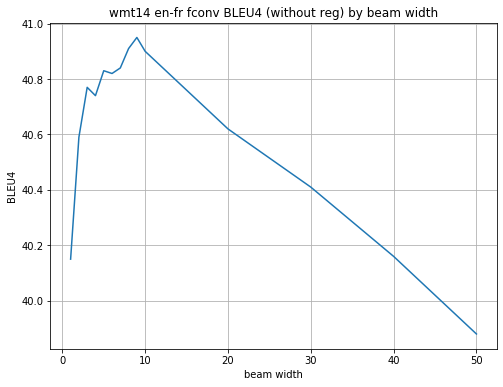
\includegraphics[width=0.7\textwidth]{fconv-bleu4.png}
		}
		\center{\caption{Зависимость BLEU4 от beam width для Convolutional seq2seq, обученной на корпусе \textit{WMT'14 English-France}}}
	\end{figure}
	
	
	Подобная проблема называется \textit{beam problem} и поднималась в статье \bibref{beam_prob1}{Somebody}{Sometm}. Далее мы подробнее разберемся в возможных причинах этого явления, пока заметим, что не исключена следующая ситуация. Пусть на некотором шаге $k_1$ beam search сохранил среди $b$ локально оптимальных префикс $s_1, \dots, s_{k_1}$, который имеет наименьшую уверенность среди всех $b$ префиксов. Пусть этот префикс построен так, что на последующих шагах найдется дополняющий его суффикс так, что итоговое предложение считается оптимальным переводом с точки зрения модели. Бывают случаи, когда такой перевод окажется некорректным. Рассмотрим такой пример. Пусть мы обучали модель перевода на корпусе сказок, исходный язык - русский, целевой язык - английский. Рассмотрим следующее предложение: \textit{Жульничество на экзамене однажды может закончиться проблемами}. Пусть наша модель выдала в качестве перевода: \textit{At the examination once upon a time}. Очевидно, что смысл перевода не соответствует исходному предложению, тем не менее это предложение оптимально с точки зрения нашей гипотетической модели. Beam problem может стать причиной таких ситуаций. Префикс \textit{At the examination once} мог попасть при широком beam search в рассмотрение и иметь низкую степень уверенности. Однако в силу того, что мы обучались на большом корпусе сказок, где встречается много примеров предложений \textit{Once upon a time...} наша модель приняла решение, что после \textit{Once} вероятно будет идти продолжение \textit{upon a time}, что привело к плохом переводу.
	
	Заметим, что в примере к плохому переводу привели некоторый особенности модели. Наша модель в качестве предсказания выдала некоторое мало вероятное в совокупности предсказания под действиям некоторых факторов. Подобные явления вызывают \textit{uncertainty}, в частности \textit{model uncertainty}, неопределенности предсказаний, вызванных моделью. Что если мы сможем построить некоторую вероятностную меру на пространстве выходных предложений $s_1, \dots, s_m$. В таком случае мы сможем оценить в совокупности насколько свойственно получить то или иное предсказание и корректировать выход модели. Задачей явного или неявного построения подобного распределения на выходах называется \textit{uncertainty estimation}. 
	
	Существуют статьи, в которых рассматриваются разные виды неопределенностей и их влияние на beam search. В данной работе мы исследуем влияние model uncertainty на beam problem. Также исследуем применимость методов uncertainty estimation в задаче машинного перевода и их влияние на результативность beam search.
	
	% Конец введения ------------------------------
	\section{Beam Search}
	\subsection{Определение метода}

	Положим префикс предсказания длины $k$:
	\begin{equation}
		f_{:k}^{i} := (f_1^{i}, \dots, f_k^{i}) \text{, \,\, где i - номер векти beam search}
	\end{equation}

	Введем следующий итеративный метод:
	
	\begin{enumerate}
		\item Подадим на вход decoder специальный токен начала предложения и скрытое состояние encoder. Получим некоторый вектор уверенностей в токенах для целевого словаря $(p_1^{00}, \dots, p_d^{00})$
		
		\item Выберем $beam$ токенов, значения уверенностей которых являются $beam$ наибольшими среди $(p_1^{00}, \dots, p_d^{00})$. Здесь $beam$ - гиперпараметр метода и называется \textit{beam width}. В итоге мы запомним: $f_{:1}^1, \dots, f_{:1}^{beam}$. 
		
		\item На следующей итерации подадим decoder в качестве входов $(f_1^{00}, \dots, f_d^{00})$ и скрытое состояние предыдущего шага. Для каждого токена мы получим свое выходное распределение $(p_1^{1i}, \dots, p_d^{1i})$ (здесь $1$ - номер итерации, $i$ - номер токена).
		\item Для всякого токена $i \in \overline{1, beam}$ рассмотрим $\forall j \in \overline{1,d}: \,\, p(f_{:1}^i) * p_j^{1i}$. Получим уверенности префиксов длины $2$. Выберем среди всех таких $beam * d$ префиксов $beam$ с наибольшими уверенностями. Запомним их: $f_{:2}^1, \dots, f_{:2}^{beam}$
		
		\item Итеративно будем продолжать операцию $\forall k \in \overline{3, m}$. Будем получать: $f_{:k}^1, \dots, f_{:k}^{beam}$
		
		\item В качестве итогового предсказания выберем $f_{:m}^i, \dots, f_{:m}^i$ такой, что его уверенность наибольшая $\forall i \in \overline{1, beam}$
	\end{enumerate} 
	
	Резюмируя, данный метод на каждой итерации декодирования хранит $beam$ "наиболее вероятных" префиксов, в отличие от наивного подхода, который жадно выбирает 1 оптимальную гипотезу на каждой итерации.
	
	\subsection{Beam Problem}
	
	В общем случае в задачах нейромашинного перевода под beam problem будем понимать явление, в результате которого, начиная с некоторого порогового значения, с ростом beam width метрика качества уменьшается при прочих равных условиях. В этой секции мы рассмотрим некоторые подходы, которые не решают проблему полностью, но значительно снижают эффект деградации метрики.
	
	В статье \bibref{corr_len_bias}{Kenton Murray}{2018} поднимаются две проблемы: beam problem и склонность моделей NMT выдавать короткие предсказания. По словам автора, решение проблемы коротких предсказаний влечет решени beam problem.
	
	В качестве демонстрации причин, которые указаны в этой статье, вызывающие beam problem, рассмотрим следующий пример из статьи.
	
	Обратимся к рис.2. Здесь представлено дерево предсказаний Beam Search для слова \textit{un hélicoptère}. Пусть ширина beam search равна 2 и на первой итерации мы сохранили две гипотезы: \textit{a} и \textit{an}. Заметим, что все 4 гипотезы далее могут быть потенциальными вариантами перевода, но \textit{a helicopter} в данном примере будет считаться грамотным переводом. Тем не менее засчет того, что \textit{autogyro} является единственным продолжением артикля \textit{an} при переводе исходного слова уверенность модели единичная и как следствие уверенность модели выдать \textit{an autogyro} равна $0.4$. В то же время вероятностная масса для токенов продолжения \textit{a} размазана среди слов: \textit{helicopter, chopper, whirlybird}. В результате уверенность для правильного перевода \textit{a helicopter} с точки зрения модели: $0.36$. По итогам, модель выдаст плохое предсказание. Чем больше мы будем брать beam width, тем выше вероятность того, что мы попадем на такую ситуацию, отсюда и вытекает потеря качества.
	
	\begin{figure}[t]
		\center{
			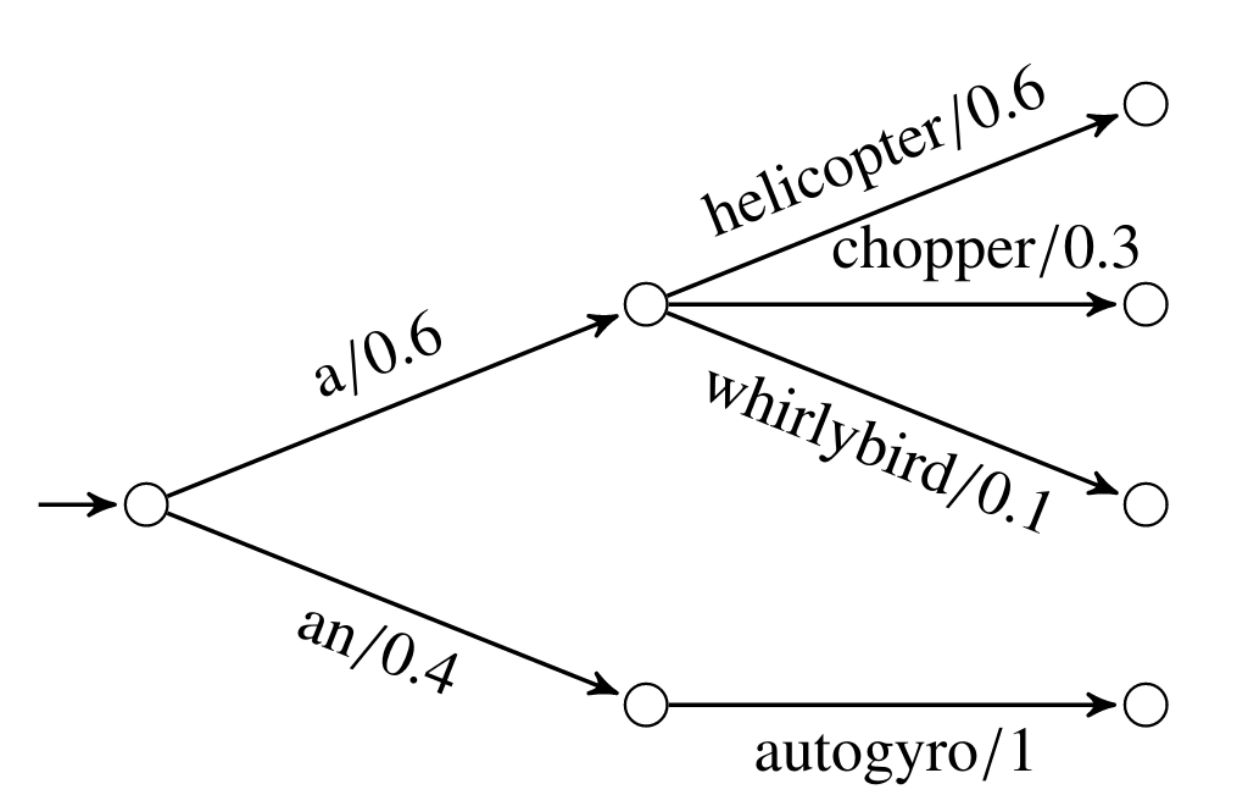
\includegraphics[width=0.5\textwidth]{helicopter.png}
		}
		\center{\caption{Label bias causes this toy word-by-word translation model to translate French helicopter incorrectly}}
	\end{figure}
	
	Заметим, что этот пример демонстрирует тот факт, что если некоторый префикс влечет суффикс с низкой энтропией, то модели свойственно игнорировать второй входной токен и предсказывать в высокой уверенностью один из нескольких высоко вероятных суффиксов. В результате низкая энтропия суффикса влечете переоценку этой ветки предсказание и как следствие плохое качество. Кроме того высока вероятность получения коротких предсказаний из-за низкой энтропии, т.к. модель начинает игнорировать некоторые токены в угоду высокой уверенности низкоэнтропийных суффиксов. По этой причине авторы статьи связывают проблему коротких предсказаний и beam problem вместе.
	
	Стандартный функционал качества для задачи машинного перевода \textit{cross-entropy}:
	\begin{equation}
		s(f) = \Sigma_{i=1}^{L}\log p(f_i | f_{:i}), \,\,\, \text{где $L$ - длина перевода}
	\end{equation}
	
	В качестве решений авторы статьи предлагают следующие корректировки функционала качества:
	\begin{enumerate}
		\item Length normalization
		\begin{equation}
			s'(f) = s(f) / L
		\end{equation}
		
		\item Google's NMT system. Length normalization
		\begin{equation}
			s'(f) = s(f) \Big/ \frac{(5 + L) ^ \alpha}{(5 + 1) ^ \alpha}
		\end{equation}
		
		\item Word reward
		\begin{equation}
			s'(f) = s(f) + \gamma L
		\end{equation}
	\end{enumerate}
	
	
		
	
	% Библиография --------------------------------
	\begin{thebibliography}{0}
		\bibitem{beam_prob1}\hypertarget{beam_prob1}{}
		Первая статья в которой поднималась проблема beam search
		\bibitem{fconv}\hypertarget{fconv}{}
		Jonas Gehring, Michael Auli, David Grangier, Denis Yarats, Yann N. Dauphin. Facebook AI Research. Convolutional Sequence to Sequence Learning. 25 Jul 2017.
		\bibitem{seq2seq}\hypertarget{seq2seq}{}
		Здесь должна быть статья по seq2seq
		
		\bibitem{corr_len_bias}\hypertarget{corr_len_bias}{}
		Kenton Murray, David Chiang. Department of Computer Science and Engineering, University of Notre Dame. Correcting Length Bias in Neural Machine Translation. 31 Aug 2018.
		
		
		\bibitem{code2seq}\hypertarget{code2seq}{}
		\href{https://openreview.net/pdf?id=H1gKYo09tX}
		{Uri Alon, Shaked Brody, Omer Levy, Eran Yahav. Code2Seq: Generating sequences from structured representations of code. In ICLR 2019.}
	\end{thebibliography}
	% ----------------------------------------------

\end{document}

